% !TeX spellcheck = en_GB

\begin{frame}{Smart Cells}
	\begin{columns}
		
		\begin{column}{0.55\textwidth}
			\begin{tcolorbox}[enhanced jigsaw, colback=white, opacityback=.4, colframe=ElixirPurple, arc=3mm, boxrule=0mm, height=0.8\textheight, valign=center, title=Smart Cell]
				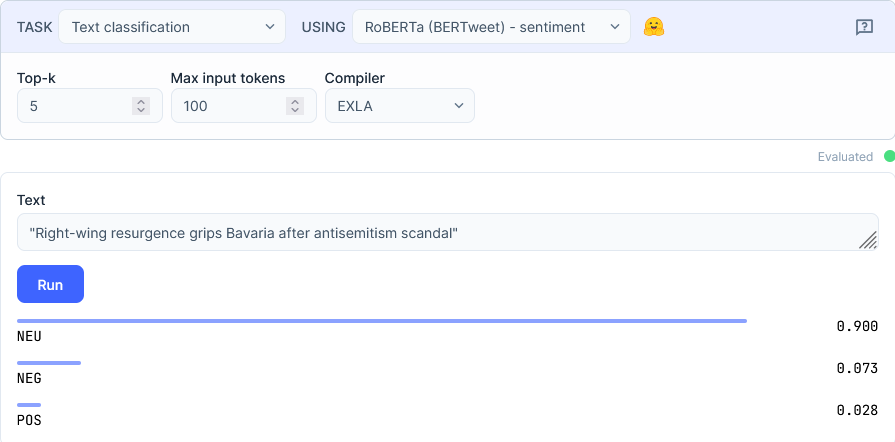
\includegraphics[width=\tcbtextwidth]{pictures/livebook/sentiment_analysis_livebook.png}
			\end{tcolorbox}
		\end{column}
		
		\begin{column}{0.55\textwidth}
			\begin{tcolorbox}[enhanced jigsaw, colback=white, opacityback=.4, colframe=ElixirPurple, arc=3mm, boxrule=0mm, height=0.8\textheight, valign=center, title=Code]
				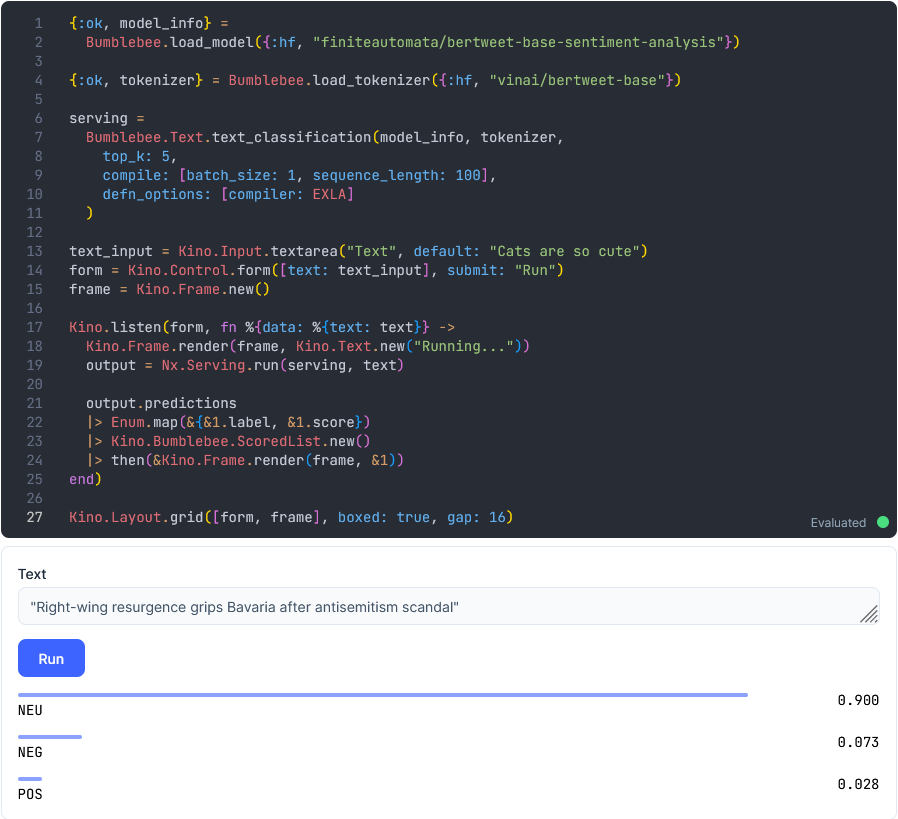
\includegraphics[height=\tcbtextheight]{pictures/livebook/sentiment_analysis_livebook_code.png}
			\end{tcolorbox}
		\end{column}
	\end{columns}
\end{frame}


\begin{frame}{Sentiment Analysis}
	\begin{columns}
		
		\begin{column}{0.55\textwidth}
			\begin{tcolorbox}[enhanced jigsaw, colback=white, opacityback=.4, colframe=ElixirPurple, arc=3mm, boxrule=0mm, height=0.8\textheight, valign=center, title=English]
				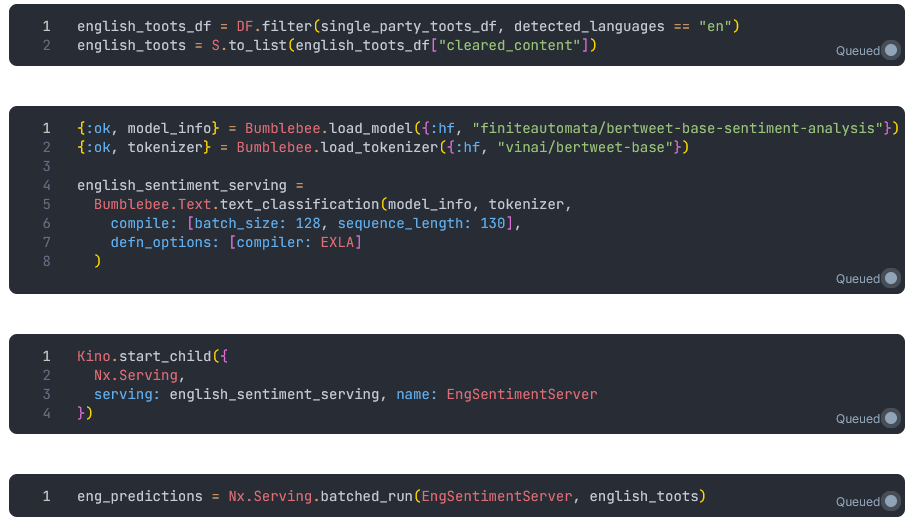
\includegraphics[width=\tcbtextwidth]{pictures/livebook/sentiment_analysis_en.png}
			\end{tcolorbox}
		\end{column}
		
		\begin{column}{0.55\textwidth}
			\begin{tcolorbox}[enhanced jigsaw, colback=white, opacityback=.4, colframe=ElixirPurple, arc=3mm, boxrule=0mm, height=0.8\textheight, valign=center, title=German]
				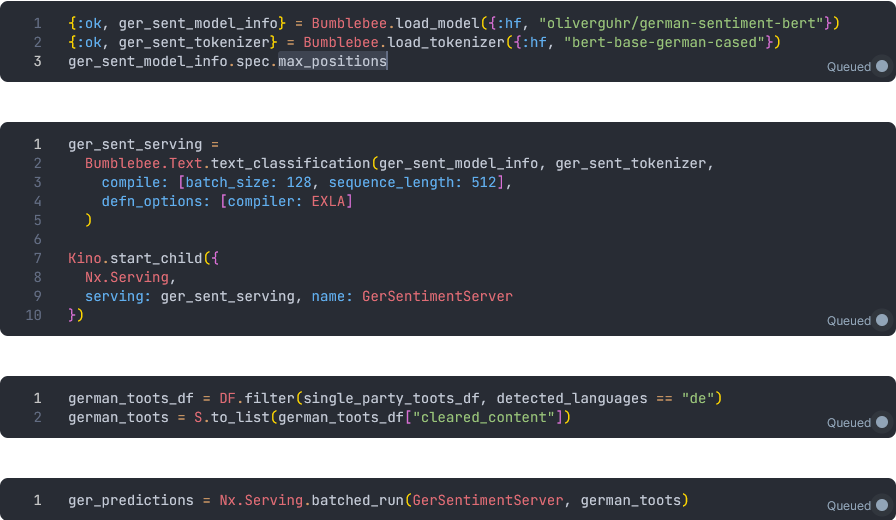
\includegraphics[width=\tcbtextwidth]{pictures/livebook/sentiment_analysis_de.png}
			\end{tcolorbox}
		\end{column}
	\end{columns}
\end{frame}



\begin{frame}{Sentiment CSU}
	\begin{figure}[htbp]
		\centering
		\includegraphics[height=0.9\textheight, keepaspectratio]{pictures/paper/sentiments/visualization\_sentiment\_csu.png}
	\end{figure}
\end{frame}





\begin{frame}{Sentiment Frei Waehler}
	\begin{figure}[htbp]
		\centering
		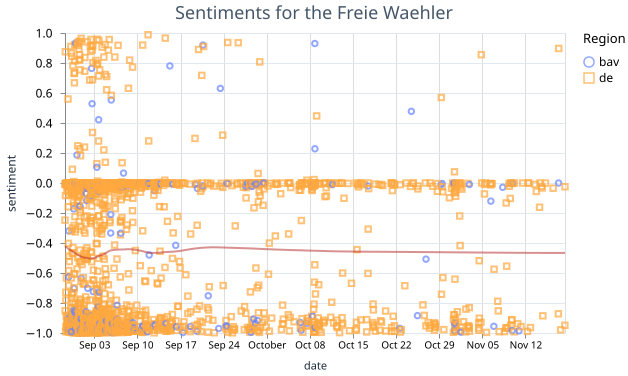
\includegraphics[height=0.9\textheight, keepaspectratio]{pictures/paper/sentiments/visualization_sentiment_fw.png}
	\end{figure}
\end{frame}


\begin{frame}{Sentiment Buendnis 90/Gruene}
	\begin{figure}[htbp]
		\centering
		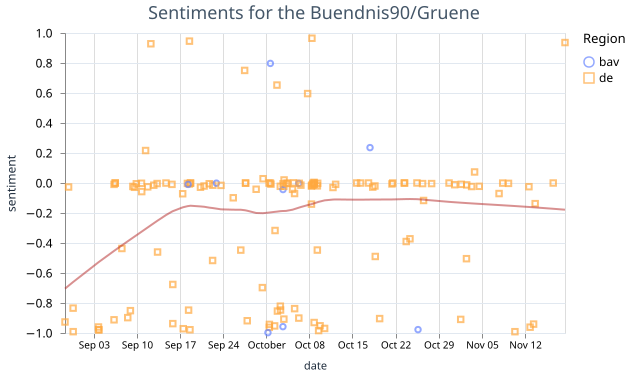
\includegraphics[height=0.9\textheight, keepaspectratio]{pictures/paper/sentiments/visualization_sentiment_gruene.png}
	\end{figure}
\end{frame}
